% Mirror: https://github.com/SIGma-UIUC/presentation-format
% --------------------------------------------------------------------
% This is a simple Beamer document that uses beamerthemesigma.sty
% Reading the comments should help you create a presentation even if
% you've never used Beamer before.
% --------------------------------------------------------------------

% Set our document class to Beamer
\documentclass[aspectratio=169, handout]{beamer}
% \documentclass[aspectratio=169, handout]{beamer}
% Add handout option to ignore pauses

% From Jeff E
\usepackage{algo}
% Some more macros
\usepackage{sigmastyle}

\usepackage{gensymb}


% Set a title
\title{Quantum Gates and Circuits}

% Set a subtitle if you desire

% Whoever worked on the presentation:
\author{Parth Deshmukh, Andrey Vlasov}

% Date looks ugly, so leave blank
\date{}
\newcommand{\twovec}[2]{\begin{pmatrix} #1 \\ #2 \end{pmatrix}}
\newcommand{\tworvec}[2]{\begin{pmatrix} #1 & #2 \end{pmatrix}}
\newcommand{\twomat}[4]{\begin{pmatrix} #1 & #2 \\ #3 & #4 \end{pmatrix}}

% An institute name, if you're so inclined
% \institute{University of Illinois Urbana-Champaign}

% Use the SIGma theme for this Beamer presentation
\usetheme{sigma}
% --------------------------------------------------------------------

% Begin document
\begin{document}

% Beamer calls each slide a "frame", defined within the environment:
% \begin{frame}
%   <frame content here>
% \end{frame}

% This frame is just the title.
\begin{frame}
\titlepage
\end{frame}

% A frame with the table of contents.
% This frame's title is "Outline".
\begin{frame}{Outline}
  \tableofcontents
\end{frame}

\begin{frame}{Important notes}
  % Let's put some real content in this frame:
  \begin{itemize}
    \item This is part 2 of 2 in a series on quantum error correction. Hopefully you enjoyed the last one!
    \item Some advice: when learning quantum mechanics, treat it like a game with rules to play. (Unless you're a physicist.)
  \end{itemize}
\end{frame}

\begin{frame}{Quick recap}
    \begin{itemize}
        \item We represent the states of qubits as vectors in $\mathbb{C}^2$ using bra-ket notation \pause
        \item We can do everything to them that we can do to vectors \pause
        \item Most importantly, we can measure them: $|\langle 0 | \psi \rangle|^2$ tells us the probability we get 0, and $|\langle 1 | \psi \rangle|^2$ the probability we get 1
    \end{itemize}
\end{frame}

\section{Quantum circuits}
\frame{\sectionpage}
\begin{frame}{What are circuits?}
    \begin{itemize}
        \item Circuits in classical computing are what EEs and CEs study \pause
        \item They have \textcolor{sigma@mainblue}{wires} that carry individual bits and \textcolor{sigma@mainblue}{gates} that take in those wires and modify their bits \pause
        \item The language of circuits is \textcolor{sigma@mainblue}{Boolean logic}
    \end{itemize}
\end{frame}

\begin{frame}{A classical circuit}
  % This is how you'd include an image, centered.
  \begin{figure}
      \centering
      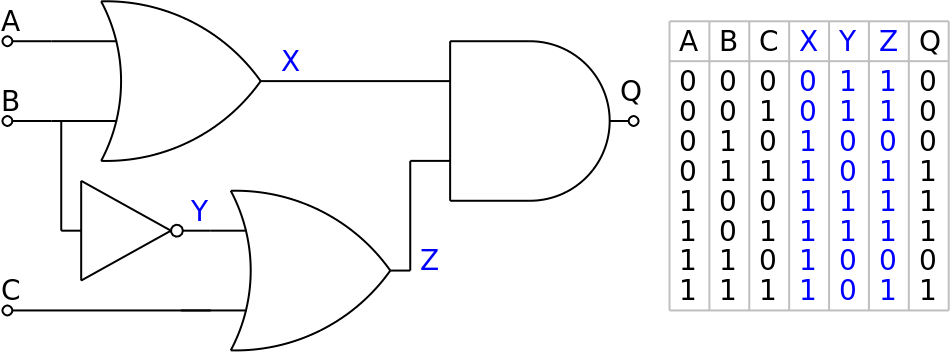
\includegraphics[width=0.8\textwidth]{combologiccirc.png}
      \caption{$X$ and $Z$ are OR, $Y$ is NOT, $Z$ is NAND (AND then NOT)}
  \end{figure}
\end{frame}

\begin{frame}{Classical to quantum circuits}
    \begin{itemize}
        \item Quantum circuits operate exactly the same way; they have wires carrying qubits and quantum gates \pause
        \item There's one important rule to contend with: \textit{we can reverse time} \pause
        \item Not actually, but the laws governing quantum mechanics are the same whether time moves forwards or backwards \pause
        \item So we need the same amount of wires going out and in, and our gates need to be reversible - in fact, they need to be \textcolor{sigma@mainblue}{unitary}
    \end{itemize}
\end{frame}

\begin{frame}{A quantum circuit}
    \begin{figure}
            \centering
            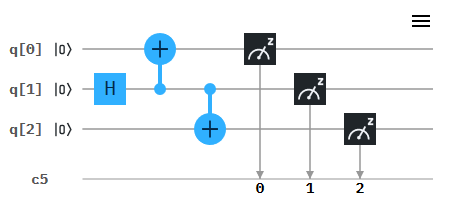
\includegraphics[width=0.8\linewidth]{Am6Sg.png}
            \caption{We have three wires going in and out, called the \textcolor{sigma@mainblue}{quantum register,} and a \textcolor{sigma@mainblue}{classical register} to collect the outcome of measurements.}
        \end{figure}
\end{frame}


% Start a section: *sections* (subsections, etc.) are what show up in the TOC.
\section{Quantum Gates}
% Section pages can be printed thus:
\frame{\sectionpage}
% There's a way to automate this, see:
% https://tex.stackexchange.com/questions/178800/creating-sections-each-with-title-pages-in-beamers-slides/178803

\begin{frame}{Basic Definition}
    \begin{itemize}
        \item A quantum gate \textit{acts} on a qubit \pause
        \item In other words, a quantum gate changes the state of a qubit \pause
        \item There are a few properties we want quantum gates to have \pause
        \item The reason for these properties: visually, single-qubit quantum gates are rotations on the Bloch sphere
    \end{itemize}
\end{frame}

\begin{frame}{Quantum Gate Properties}
    \begin{itemize}
        \item Recall that a quantum state of a qubit is given by a superposition of our chosen ONB \pause
        \item In quantum physics, we want the total probability to always be equal to 1 \pause
        \item Therefore, when the state of a qubit changes, we want the change to be \textit{ditsributive} across superpositions and \textit{normalized} \pause
        \item Thus every quantum gate $U$ must be a normalized linear map
    \end{itemize}
\end{frame}

\begin{frame}{What is a linear map?}
    \begin{itemize}
        \item Roughly, a function that preserves operations and linear combinations \pause
        \item Recall that a quantum state is a linear combination of our two basis states \pause
        \item $U(\alpha | 0 \rangle + \beta | 1 \rangle)=\alpha U(| 0 \rangle) + \beta U(| 1 \rangle)$ \pause
        \item Normalization: $|\alpha|^2 + |\beta|^2 = 1$
    \end{itemize}
\end{frame}

\begin{frame}{Why is it called $U$?}
    \begin{itemize}
        \item Every valid quantum gate can be represented as a $U$nitary matrix, and every unitary matrix is a quantum gate \pause
        \item In bra-ket notation, $\langle\psi|\psi\rangle=\psi^{*^\intercal}\psi=1$ by Born's Rule \pause
        \item A unitary matrix is defined as $U^{*^\intercal}U=U^{\dagger}UI$ \pause 
        \item $\langle U\psi|=(|U\psi\rangle)^{\dagger}=(U|\psi\rangle)^{\dagger}=|\psi\rangle^{\dagger}U^{\dagger}=\langle\psi|U^{\dagger}$ \pause
        \item $\langle U\psi|U\psi\rangle=\langle\psi|U^{\dagger}U|\psi\rangle=\langle\psi|\psi\rangle=1$
    \end{itemize}
\end{frame}

\subsection{Specific Gates}
% Section pages can be printed thus:
\frame{\subsectionpage}

\begin{frame}{The Hadamard Gate}
    \begin{itemize}
        \item $H|0\rangle = |+\rangle$, $H|1\rangle = |-\rangle$ \pause
        \item Like any quantum gate, the Hadamard gate is reversible \pause
        \item $H|+\rangle = |0\rangle$, $H|-\rangle = |1\rangle$ \pause
        \item Corresponds to a $180\degree$ rotation about the $x+z$-axis on the Bloch sphere \pause
        \item So $H^2$ is a $360\degree$ rotation, which is just $I$
    \end{itemize}
\end{frame}

\begin{frame}{Understanding the Hadamard gate}
    \begin{itemize}
        \item The actual Hadamard gate is $H = \frac{1}{\sqrt{2}}\twomat{1}{1}{1}{-1}$ \pause
        \item If we let the Hadamard gate act on a qubit $|0 \rangle$ and then measure it, what do we get? \pause
        \item The changed qubit is written as $H|0\rangle,$ and if we measure it, our probabilities are written $|\langle 0 | H | 0 \rangle|^2$ and $|\langle 1 | H | 0 \rangle|^2$ \pause
        \item If we work it out, we get exactly 1/2 for both! Remember that $H|0\rangle = |+\rangle,$ so we get $|\langle 0 | + \rangle|^2 = (\frac{1}{\sqrt{2}})^2$ (and same for $|\langle 1 | + \rangle|^2$) \pause
        \item This also works for $|1\rangle,$ so the point of the Hadamard gate is to put a qubit exactly between $|0\rangle$ and $|1\rangle$ on the Bloch sphere
    \end{itemize}
\end{frame}

\begin{frame}{The Pauli-X gate}
    \begin{itemize}
        \item Another useful single-qubit gate \pause
        \item Represented as $X = \twomat{0}{1}{1}{0}$ \pause
        \item The Pauli-X gate is simply a 180 degree rotation about the X axis of the Bloch sphere \pause
        \item Which means it's a bit flip: $X|0\rangle = |1\rangle,$ and $X|1\rangle = |0\rangle$
    \end{itemize}
\end{frame}

\begin{frame}{Multiple-qubit gates}
    \begin{itemize}
        \item Gates can operate on more than one qubit: for example, CNOT operates on two gates, and CCNOT operates on three \pause
        \item These are represented as 4x4 and 8x8 matrices, respectively, which are unitaries in the wider spaces $\mathbb{C}^4$ and $\mathbb{C}^8$ \pause
        \item Why are we doing this? Because the input qubits to multi-qubit quantum gates need to be combined with the tensor product, since they could become entangled \pause
        \item Example: input qubits $|0\rangle$ and $|1\rangle,$ so the input to the CNOT gate would be the tensor product $|01\rangle = \twovec{1}{0} \otimes \twovec{0}{1} = \begin{pmatrix}
            0 \\ 1 \\ 0 \\ 0
        \end{pmatrix}$
    \end{itemize}
\end{frame}

\begin{frame}{The CNOT gate}
    \begin{itemize}
        \item CNOT = controlled-NOT \pause
        \item Flips the second qubit only if the first qubit is $|1\rangle,$ does nothing if it's $|0\rangle$ \pause
        \item CNOT gate is defined then as $CNOT = \begin{pmatrix}
        1 & 0 & 0 & 0 \\
        0 & 1 & 0 & 0 \\
        0 & 0 & 0 & 1 \\
        0 & 0 & 1 & 0
    \end{pmatrix}$
        \item First qubit is the control qubit, second qubit is the target qubit \pause
        \item If we have different qubits than $|0\rangle$ and $|1\rangle$, the behavior is analogous but more complex
    \end{itemize}
\end{frame}

\begin{frame}{CNOT entanglement}
    \begin{itemize}
        \item CNOT gates are super useful to entangle bits together \pause
        \item Since they're the simplest gate that acts on two qubits, they're the simplest way to tie two qubits together - which is where the power of quantum algorithms lie \pause
        \item The simplest way of making a maximally entangled state uses a Hadamard and CNOT to make what's called the \textcolor{sigma@mainblue}{Bell state}
    \end{itemize}
\end{frame}

\begin{frame}{Creating the Bell state}
  % This is how you'd include an image, centered.
  \begin{figure}
      \centering
      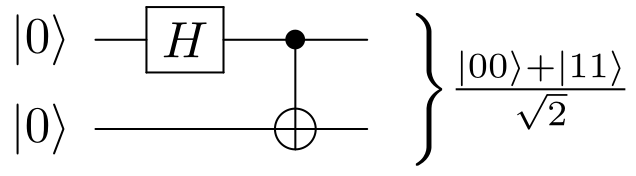
\includegraphics[width=0.8\textwidth]{bellstate.png}
  \end{figure}
\end{frame}

\section{Putting it all together}
\frame{\sectionpage}

\begin{frame}{Our goal}
    \begin{itemize}
        \item Recall we want to find a way to do quantum error correction \pause
        \item If a qubit is at $|0\rangle$ or $|1\rangle$ and drifts from it, that's a partial or complete bit flip \pause
        \item We'll use backup qubits, CNOT and Pauli-X gates, and measurement to indirectly force the qubit back onto $|0\rangle$ or $|1\rangle$ and then correct the error
    \end{itemize}
\end{frame}

\begin{frame}{The circuit}
\begin{center}
    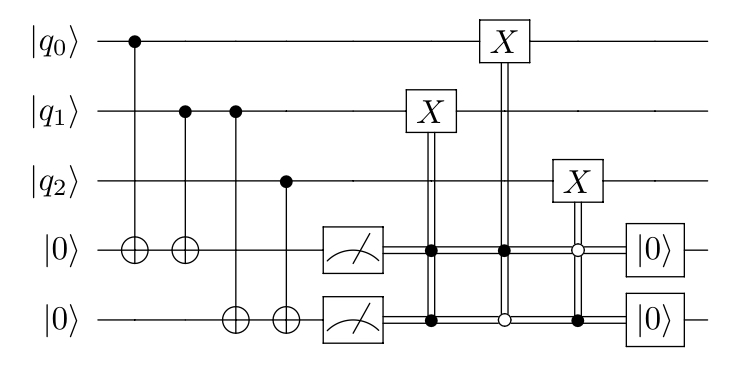
\includegraphics[width=0.8\textwidth]{bitflipcode.png}\nocite{site:xkcd}
\end{center}
\end{frame}

\begin{frame}{Step 1: encoding a qubit}
    \begin{itemize}
        \item We'll use three physical qubits to encode each logical qubit \pause
        \item If our starting qubit is $|\psi\rangle = \alpha|0\rangle + \beta|1\rangle,$ we want to turn it into $\alpha|000\rangle + \beta|111\rangle$ \pause
        \item This isn't shown in the figure, but we can do this with two CNOT gates:
    \end{itemize}
    \begin{figure}
        \centering
        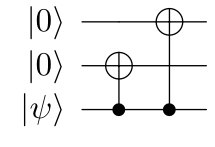
\includegraphics[width=0.3\textwidth]{kintroduction-to-classical-and-quantum-computing-1e3p 2023-10-09 20_15_18.png}
    \end{figure} \pause
    \begin{itemize}
        \item Note we're not cloning our qubit, so we respect no-cloning theorem
    \end{itemize}
\end{frame}

\begin{frame}{The circuit}
\begin{center}
    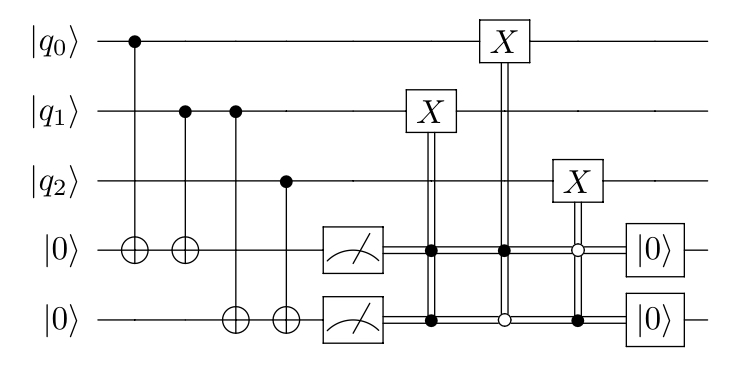
\includegraphics[width=0.8\textwidth]{bitflipcode.png}\nocite{site:xkcd}
\end{center}
\end{frame}

\begin{frame}{Step 2: measuring parities}
\begin{itemize}
    \item $|q_0\rangle, |q_1\rangle, \text{ and }|q_2\rangle$ are the three qubits from our encoded qubit $|\psi\rangle$ \pause
    \item The parity of two bits is 1 if they differ, and 0 if they don't \pause
    \item The parity of two bits is their XOR $a \oplus b.$ We implement this with CNOT, since $CNOT|a\rangle |b\rangle = |a\rangle |a \oplus b\rangle$, and put it in an backup qubit \pause
\end{itemize}
\begin{figure}
    \centering
    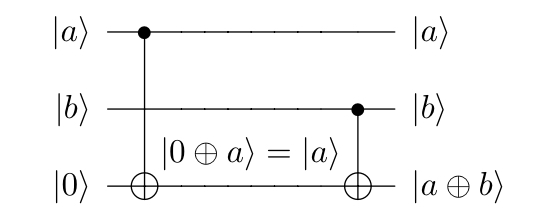
\includegraphics[width=0.5\textwidth]{sciusdknwdkn 2023-10-09 20_18_53.png}
\end{figure}
\end{frame}

\begin{frame}{The circuit}
\begin{center}
    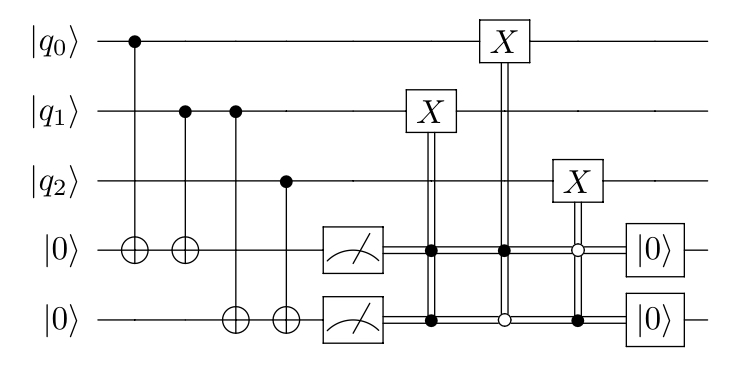
\includegraphics[width=0.8\textwidth]{bitflipcode.png}\nocite{site:xkcd}
\end{center}
\end{frame}

\begin{frame}{Step 3: measuring parities}
    \begin{itemize}
        \item We measure parities twice, so our two backup (ancilla) qubits have the parities $|q_0\rangle \oplus |q_1\rangle$ and $|q_1\rangle \oplus |q_2\rangle$ \pause
        \item If the parities are \{0, 0\}, no qubits have flipped \pause
        \item If they're \{1, 0\}, the left one has flipped \pause
        \item If they're \{0, 1\}, the right one has flipped \pause
        \item If they're \{1, 1\}, the middle one has flipped \pause
        \item We check the parities by measuring both ancilla qubits, so we don't measure our original qubit \pause
        \item The measurement has an additional benefit: it forces partial bit flips to disappear or become complete bit flips 
    \end{itemize}
\end{frame}

\begin{frame}{The circuit}
\begin{center}
    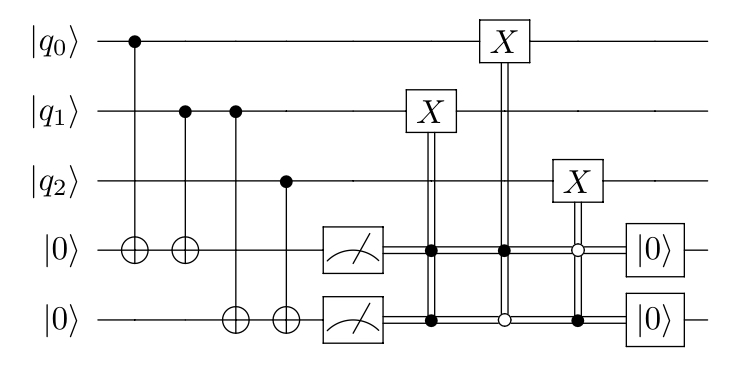
\includegraphics[width=0.8\textwidth]{bitflipcode.png}\nocite{site:xkcd}
\end{center}
\end{frame}

\begin{frame}{Step 4: correcting the error}
    \begin{itemize}
        \item Remember Pauli-X gates act as bit-flips \pause
        \item We put a Pauli-X on each physical qubit $|q_0\rangle, |q_1\rangle, |q_2\rangle$ and just flip it depending on what the parities tell us \pause
        \item The X gates are controlled with the two ancilla qubits \pause
        \item The X gate is classically the NOT gate, so this is actually the CCNOT gate
    \end{itemize}
\end{frame}

\begin{frame}{The circuit}
\begin{center}
    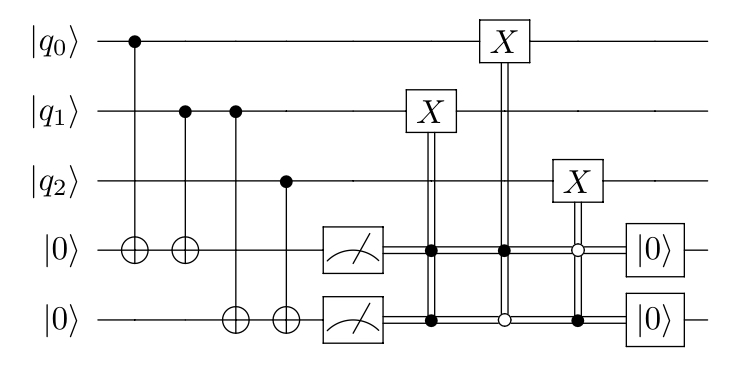
\includegraphics[width=0.8\textwidth]{bitflipcode.png}\nocite{site:xkcd}
\end{center}
\end{frame}

\begin{frame}{Phase-flip code}
    \begin{itemize}
        \item To correct phase-flips, we take advantage of the Hadamard gate \pause
        \item Phase-flips are errors in the ONB \{$|+\rangle, |-\rangle\}$, which the Hadamard gate converts to $\{|0\rangle, |1\rangle\}$ \pause
        \item We simply convert the ONB with Hadamards, run the algorithm to calculate bit parities, convert back, and use Pauli-Z gates to correct the errors
    \end{itemize}
\end{frame}

\begin{frame}{The phase-flip circuit}
    \begin{figure}
        \centering
        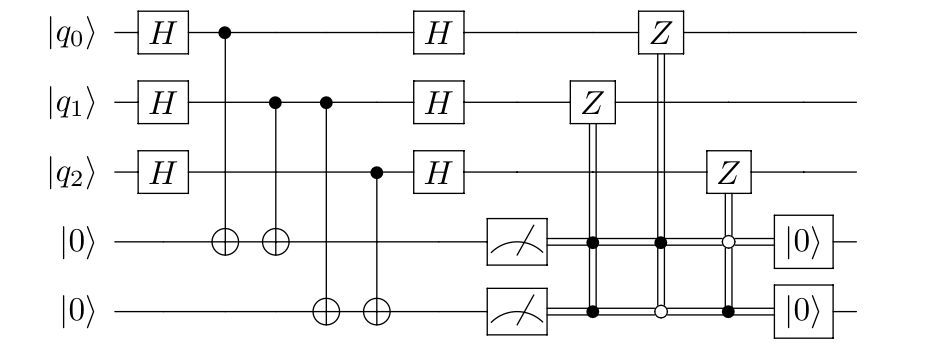
\includegraphics[width=0.8\textwidth]{phaseflipcode.png}
    \end{figure}
\end{frame}
% Asking questions is fun but we should answer some first
\begin{frame}{}
      \begin{center}
    {\color{sigma@mainblue} \LARGE Questions?}
  \end{center}
\end{frame}

% Quotes are fun, find some to use!
\font\eightss=cmssq8
\font\eightssi=cmssqi8
\newcommand\quoteAuthorDate[2]{\begingroup
  \baselineskip 10pt
  \parfillskip 0pt
  \interlinepenalty 10000 % not needed in example
  \leftskip 0pt plus 40pc minus \parindent
  \let\rm=\eightss
  \let\sl=\eightssi
  \everypar{\sl}#1\par
  \nobreak\smallskip
  \noindent\rm--- #2
  \endgroup}
% If someone can figure out how to horizontally center this and make the text bigger that'd be cool
\begin{frame}
    \begin{center}
        \item \quoteAuthorDate{Nothing can create something all the time due to the laws of quantum mechanics, and it's - it's fascinatingly interesting.}{LAWRENCE M. KRAUSS}
    \end{center}
\end{frame}

% Remove this slide if you came up with all the material yourself
\begin{frame}{Bibliography}
    \bibliography{refs}
    \bibliographystyle{alpha}
\end{frame}

\end{document}